\section{Concurrency Modelle}
Die Basis eines reaktiven Systems ist das zugrundeliegende Concurrency Modell. Ein reaktives System besteht aus vielen isolierten Komponenten, die asynchron miteinander kommunizieren. Diese Komponenten können in einem Computercluster verteilt sein und arbeiten zudem weitestgehend unabhängig voneinander und parallel. Die Programmierung von stark nebenläufigen Anwendungen durch systemnahe Konzepte, wie Threads und Locks ist aufgrund von \textit{shared memory} und dessen Synchronisation (siehe \fullref{subsec:sharenothing}) kompliziert und fehleranfällig~\cite[S.~72]{erb_concurrent_2012}.\\
Im diesem Kapitel werden zwei Concurrency Modelle erklärt, die die Komplexität nebenläufiger Anwendungen isolieren und abstrahieren. Sowohl die ereignisbasierte Concurrency, als auch die Actor-basierte Concurrency arbeitet asynchron und nicht blockierend. Um deren Funktionalität aufrecht zu erhalten ist es erforderlich, dass das darauf aufbauende System ebenfalls asynchron und nicht blockierend arbeitet~\cite[S.~171]{kuhn_reactive_2015}.

\subsubsection{Asynchrone Datenübertragung}\label{subsec:async-io}
Im vorangegangen Kapitel wurde erläutert, dass die Kommunikaktion zwischen den Komponenten asynchron erfolgen muss (siehe \ref{subsec:communication}). Jedoch ist traditionellerweise der schreibende und lesende Zugriff auf Ressourcen, wie Netzwerk oder Festplatte synchron und blockierend. Das bedeutet, die Anwendung bzw. der Thread ist für die gesamte Dauer des Zugriffs ausschließlich mit beispielsweise dem Abspeichern einer großen Datei beschäftigt.\\
\textit{Asynchronous I/O} ist ein Mechanismus moderner Betriebsysteme, welcher den asynchronen und nicht blockierenden Zugriff auf Ressourcen, wie Netzwerk, Arbeitsspeicher oder Festplatte ermöglicht.

\pagebreak

Folgende Abbildung (\ref{fig:async-io}) zeigt einen typischen Ablauf einer asynchronen und nicht blockierenden Datenübertragung. Dieses Modell erlaubt Anwendungen, die gleichzeitige Bearbeitung von Datenübertragungen und weiteren Berechnungen. 

\begin{figure}[H]
 \centering
 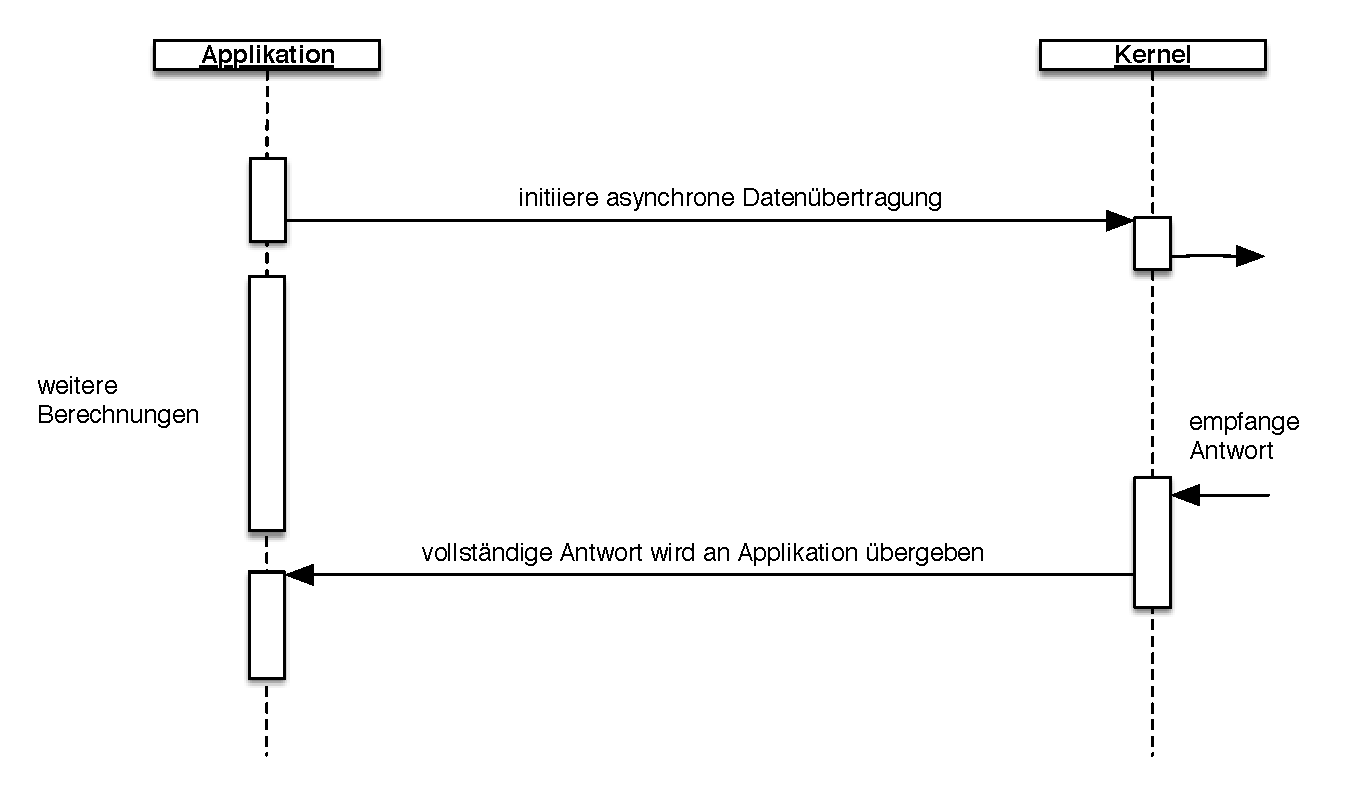
\includegraphics[width=1.0\textwidth]{4-Hauptteil/async-io/async-io.eps}
 \caption{Ablauf einer asynchronen und nicht blockierenden Datenübertragung}
 \label{fig:async-io}
\end{figure}

Die Anwendung kann nach der Initiierung der Datenübertragung sofort mit weiteren Berechnungen fortfahren. Das Betriebssystem informiert die Anwendung über die erfolgreiche Übertragung und übergibt die vollständige Antwort an die Anwendung. Durch diesen Mechanismus ist es möglich mit einem Thread mehrere Datenübertragungen asynchron abzuarbeiten, da diese den Thread nicht, wie traditionellerweise blockieren~\cite{jones_boost_2006}.

\pagebreak

Eine Webapplikation ist meist stark an Datenübertragung gebunden. Sei es die eigentliche HTTP Schnittstelle, der Zugriff auf die Datenbank oder die Kommunikation mit anderen Services. Eine Anfrage hat meist zur Folge, dass auf eine Datenbank zugegriffen wird. Die Ergebnisse der Datenbankanfrage werden aufbereitet und an den Client zurückgegeben. Der eigentliche Aufwand für die CPU ist relativ gesehen sehr gering.\\
Eine traditionelle Multi-threaded Webapplikation weist jeder eingehenden Anfrage einen dedizierten Thread zu. Mit synchroner und blockierender Datenübertragung ist dieser Thread so lange blockiert, bis die Antwort auf die Anfrage beim Client eingegangen ist. Ein Client mit einer langsamen Netzwerkanbindung blockiert deshalb einen Thread länger, als ein Client mit einer schnellen Netzwerkanbindung.\\
Um eine Multi-threaded Webapplikation skalieren zu können, setzt man Thread-Pools ein, die eine Vielzahl von Threads vorhalten --- meist weit aus mehr als der Prozessor Kerne hat. Jedoch ist die Koordination der Threads aufwendig und hat häufiges \textit{context switching} zur Folge.\\
Mit dem Modell der asynchronen und nicht blockierenden Datenübertragungen lassen sich Ressourcen effizienter nutzen. Zudem erhält man eine bessere vertikale Skalierung, als beispielsweise beim beschriebenen \enquote{One thread per request} Modell~\cite[S.~171]{butcher_seven_2014}~\cite[S.~76]{erb_concurrent_2012}.

\pagebreak

\subsection{Ereignisbasierte Concurrency}\label{subsec:eventdriven-concurrency}
Viele Anwendungen nutzen das Konzept der Events, um den Ablauf der Ausführung zu steuern. Man spricht auch von ereignisorientierter Software.\\ 
Ein Event ist ein Ereignis respektive ein Signal über eine Zustandsänderung. Im Gegensatz zu einer Nachricht hat ein Event keinen expliziten Empfänger, also keine Zieladresse. Komponenten können sogenannte Event-Handler an einem System registrieren. Diese werden dann über Zustandsänderungen informiert bzw. aufgerufen. Solange es zu keiner Zustandsänderung kommt, wird auch kein Event-Handler aufgefordert, ein Event zu verarbeiten und bleibt somit inaktiv~\cite[S.~91]{erb_concurrent_2012}.

\subsubsection{Reactor Pattern}
Ereignisorientierte Anwendungen müssen in der Regel viele Events von vielen verschiedenen Quellen koordinieren und abarbeiten. Beispielsweise ist jede Anfrage an eine Webanwendung ein Event und jeder Client folglich eine Quelle. Die Anfragen bzw. die Events können auch parallel bei der Anwendung eintreffen.\\
Um die Events abzuarbeiten, wird oft auf das Reactor Pattern zurückgegriffen (\autoref{fig:event-loop}). Events aus verschiedensten Quellen werden serialisiert und Event für Event abgearbeitet bzw. an die entsprechenden Event-Handler übergeben. Die Ausführung der Event-Handler erfolgt synchron. Die Reactor Komponente arbeitet in einer Endlosschleife, genannt Event loop~\cite[S.~260~-~S.~261]{buschmann_pattern_2011}.

\begin{figure}[H]
 \centering
 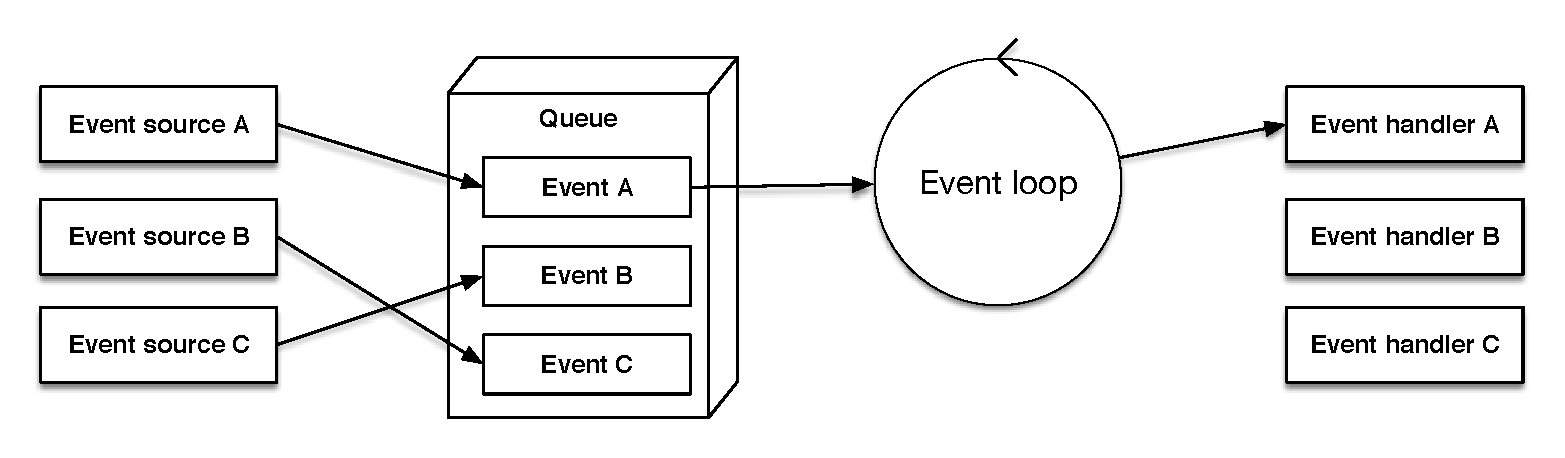
\includegraphics[width=0.9\textwidth]{4-Hauptteil/event-loop/event-loop.eps}
 \caption{Graphische Darstellung der Funktionsweise des Reactor Patterns}
 \label{fig:event-loop}
\end{figure}

Die Event-Loop wird typischerweise von genau einem Thread ausgeführt. Um dennoch nebenläufig mehrere Anfragen verarbeiten zu können, nutzt man Asynchronous~I/O (siehe~\ref{subsec:async-io}). So ist es möglich nebenläufig, mit nur einem Thread, auf Events von vielen verschiedenen Quellen zu reagieren. Ein Event-Handler blockiert während der synchronen Ausführung den Thread der Event-Loop und somit die Abarbeitung weiterer Events. Folglich ist das Reactor-basierte Concurrency Modell vorallem für datenübertragungsintensive Applikationen, die von Asynchronous I/O profitieren, sinnvoll~\cite[S.~73]{kuhn_reactive_2015}~\cite[S.~92]{erb_concurrent_2012}. Sollte es dennoch langwierige Operationen während der Abarbeitung von Events geben, ist es möglich diese in zusätzliche Worker-Threads auszulagern, um die Event-Loop nicht zu blockieren.\\
Mit dem Reactor Pattern ist es möglich viele Anfragen nebenläufig, mit nur einem Thread, zu verarbeiten. Es entsteht kein Performance Overhead, wie bei traditionellen \enquote{One thread per request} Applikationen. Zudem wird die Komplexität der nebenläufigen Verarbeitung in der Reactor Komponente gekapselt und der Entwickler muss nicht mit den typischen Problemen der nebenläufigen Programmierung kämpfen. Außerdem können Event-Handler leicht wiederverwendet und kombiniert werden.\\
Es gibt zwei populäre Implementierungen dieses Concurrency Modells. Zum einen das JavaScript (V8) basierte Node.js\footnote{https://nodejs.org} und zum anderen das JVM basierte Vert.x\footnote{http://vertx.io}. Beide implementieren das Reactor Pattern --- unterscheiden sich jedoch in ihrer Anwendbarkeit für reaktive Anwendungen.\\
Vert.x bietet dem Entwickler die Möglichkeit über einen verteilten Event Bus eine Applikation \textit{message-driven} zu implementieren. Zudem skaliert Vert.x auf einem Multi-core Prozessor besser, wie das Single-Threaded Node.js. Vert.x startet in der Standardeinstellung mehrere Event loops --- so viele, wie der Prozessor Cores hat --- und nennt dieses Konzept Multi-Reactor Pattern. Durch diese beiden Mechanismen, dem verteilten Event Bus, sowie dem Multi-Reactor Pattern, ist es möglich vertikal und horizontal zu skalieren. Unter diesen Gesichtpunkten eignet sich Vert.x als Basis Framework zur Entwicklung von reaktiven Anwendungen~\cite[S.~74]{kuhn_reactive_2015} \cite[S.~93~\&~S.~94]{erb_concurrent_2012}.

\pagebreak

\subsection{Actor-basierte Concurrency}\label{subsec:actor-model}
Im folgenden Abschnitt wird ein weiteres Concurrency Modell als Basis für reaktive Software vorgestellt.\\
Actor-basierte Concurrency oder kurz das \enquote{Actor Modell} stammt ursprünglich von Dr. Carl Hewitt et al. aus dem Jahr 1973~\cite{hewitt_universal_1973}. Die grundlegende Idee des Actor Modells, ist die Abstraktion der Concurrency durch asynchronen Nachrichtenaustausch zwischen Komponenten. Eine Komponente in einer Actor-basierten Anwendung wird Actor genannt. Alan Kay, bekannt für seine Pionierarbeit zu objektorientierter Programmierung und außerdem einer der Entwickler der einflussreichen Sprache Smalltalk, sagte in einem Interview folgendes über das Actor Modell~\cite{binstock_interview_2012}:

\begin{quotation}
[...] the Actor model retained more of what I thought were the good features of the object idea [...]
\end{quotation}

Kay bezog sich dabei auf die geläufige Interpretation objektorientierter Programmierung, wie sie beispielsweise in C++ oder Java umgesetzt wurde. Der Kerngedanke der objektorientierten Programmierung müsste vielmehr die Kommunikation zwischen den Komponenten sein und sollte den Fokus nicht auf die Attribute oder das innere Verhalten der Objekte legen~\cite[S.~10]{vernon_reactive_2016}.\\
Das Actor Modell setzt im Grunde an diesem Gedanken an und lässt Komponenten über Nachrichten kommunizieren. 

\begin{figure}[H]
 \centering
 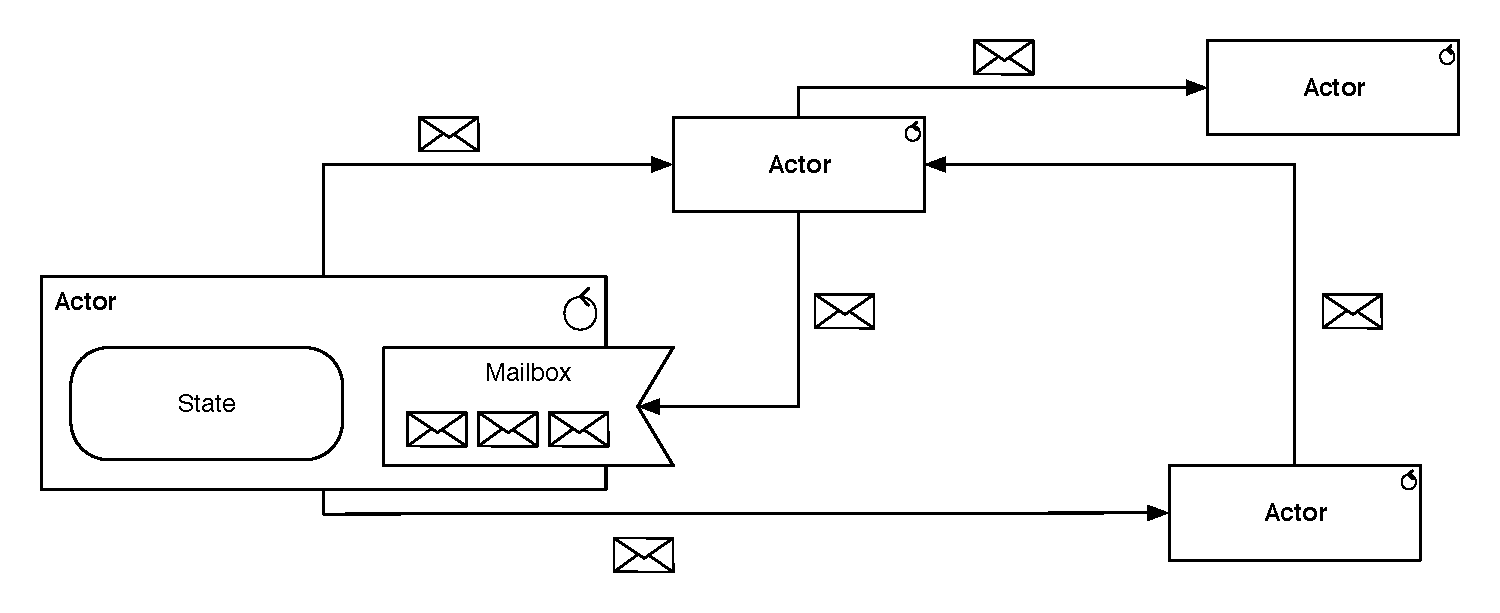
\includegraphics[width=1.0\textwidth]{4-Hauptteil/actor-model/actor-model.eps}
 \caption{Graphisches Beispiel einer Actor-basierten Anwendung.}
 \label{fig:actor-model}
\end{figure}

Ein Actor ist die kleinste logische Einheit in einer Actor-basierten Anwendung im Sinne des \enquote{Single Responsibility Principle} (siehe \ref{subsec:simple-component-pattern}), wie das graphische Beispiel eines Bestellvorgangs (\autoref{fig:actor-model}) zeigen soll~\cite[S.~13]{vernon_reactive_2016}. Hewitt sagte, dass ein einzelner Actor kein Actor System sei. Parallelität in einem Actor System wird erst durch eine Vielzahl von Actors ermöglicht \cite[S.~15]{vernon_reactive_2016}. Ein Actor ist leichtgewichtig und benötigt nur Rechenkapazität, wenn Nachrichten verarbeitet werden.\\
Jeder Actor besitzt eine sogenannte Mailbox, diese dient als Zwischenspeicher für eingehende Nachrichten. Außerdem hat jeder Actor einen Namen bzw. eine Adresse. Um einem Actor eine Nachricht zu schicken, wird die Adresse des Actors benötigt. Diese ermöglicht es, mit einem Actor über eine abstrakte Referenz zu interagieren und dies wiederum ermöglicht \textit{location transparency}. Die Übertragung einer Nachricht an die Mailbox ist von unbestimmter Dauer und erfolgt asynchron. Zudem wird keine erfolgreiche Zustellung der Nachrichten garantiert \cite[S.~84]{erb_concurrent_2012} \cite[S.~83]{kuhn_reactive_2015}.\\
Ein Actor arbeitet jede Nachricht aus der Mailbox sequenziell ab. Deshalb muss während der Verarbeitung nicht auf Probleme bzgl. Nebenläufigkeit geachtet werden~\cite[S.~14]{vernon_reactive_2016}.\\
Ein Actor kann auf drei verschiedene Weisen auf eine Nachricht reagieren \cite[S.~84]{erb_concurrent_2012}:

\begin{enumerate}
\item Ein Actor kann eine begrenzte Anzahl von Nachrichten an andere Actors schicken.
\item Ein Actor kann eine begrenzte Anzahl weiterer Actors erzeugen.
\item Ein Actor kann den eigenen internen Zustand ändern.
\end{enumerate}

Der Zustand eines Actors ist isoliert und kann nur von dem Actor selbst verändert werden. Zustandsänderungen und daraus resultierende Verhaltensänderungen wirken sich aufgrund der sequenziellen Abarbeitung erst auf nachfolgende Nachrichten aus. Aufgrund dieser Voraussetzung kann man mit einem Actor problemlos endliche Automaten implementieren \cite[S.~14]{vernon_reactive_2016} \cite[S.~84]{kuhn_reactive_2015}.\\
Actor-basierte Anwendungen setzen somit auf \textit{mutable state} --- jedoch wird dieser nicht geteilt. Ein Actor kapselt seinen Zustand und interagiert nur über Nachrichten mit anderen Actors (siehe \fullref{subsec:sharenothing}). Der isolierte Zustand und die sequenzielle Verarbeitung der Nachrichten ermöglichen außerdem die sogenannte \enquote{lock-free concurrency} innerhalb eines Actors \cite[S.~85]{kuhn_reactive_2015}.\\
Eine Actor-basierte Anwendung besteht aus vielen Actors. Zudem entsteht durch die o.g. zweite Eigenschaft, weitere Actors zu erzeugen, eine Actor Hierachie. Komplexe Prozesse werden aufgebrochen und jeder Actor ist für eine kleine Aufgabe bzw. einen Task im System zuständig.\\
Die Hierarchie ermöglicht es, dass Konzept der \textit{supervision} umzusetzen. Übergeordnete Actors sind für Koordination und Verteilung der Tasks via Nachrichten verantwortlich. Tasks werden an untergeordnete Actors delegiert. Zudem übernehmen übergeordnete Actors eine Kontrollfunktion. Verhält sich ein untergeordneter Actor fehlerhaft werden Maßnahmen, wie beispielsweise ein Neustart des fehlerhaften Actors, ergriffen. Ein Actor kann Fehler seiner untergeordneten Actors auch weiter nach oben propagieren, um dem System die Möglichkeit zu geben, Fehler zu beheben~\cite[S.~15]{vernon_reactive_2016} \cite[S.~83]{kuhn_reactive_2015} \cite[S.~86]{erb_concurrent_2012}.\\

Das Actor Modell wurde poplär durch die Programmiersprache Erlang\footnote{https://www.erlang.org/} und das Framework Akka\footnote{http://akka.io}. Diese Actor Systeme abstrahieren die Koordination der parallelen Ausführung. Die Verarbeitung einer Nachricht innerhalb eines Actors erfolgt immer durch maximal einen Thread. Während dieser Verarbeitung ist ein Thread ausschließlich für einen spezifischen Actor zuständig. Ein Actor und ein Thread sind jedoch nicht aneinander gebunden. Folglich ist es möglich, ein Actor System mit beispielsweise tausenden Actors ressourcenschonend zu betreiben.\\
Die Erlang VM startet beispielsweise einen Thread-Pool mit so vielen Threads, wie Rechenkerne zur Verfügung stehen. Diese Threads werden nun Actors zugewiesen, deren Mailboxen Nachrichten enthalten. Aufgrund der limitierten Ressourcen darf ein Actor einen Thread nicht für immer blockieren. Deshalb ist \textit{Asynchronous I/O}, wie bei der ereignisbasierten Concurrency (\ref{subsec:eventdriven-concurrency}), für das Actor Modell vorteilhaft. Durch Scheduling, wie man es auch von Betriebssystemen kennt, achtet das Actor System auf Fairness, um \textit{starvation} einzeler Actors zu verhindern.\\

Mit einer Actor-basierten Anwendung ist es möglich, eine Applikation \textit{message-driven} zu entwickeln. Beide Implementierungen, sowohl Erlang als auch Akka unterstützen die Verteilung von Actors auf mehrere Nodes und vorallem die Kommunikation via Nachrichten über mehrere Nodes hinweg. Somit skalieren Actor-basierte Systeme horizontal und vertikal. Bezüglich \textit{resilience} bietet die Actor Hierachie und das Konzept der \textit{supervision} eine gute Basis, um eine Anwendung von vornherein \textit{resilient} zu entwerfen.\\

Beide Modelle, sowohl die ereignisbasierte als auch die Actor-basierte Concurrency, bieten je nach Implementierung essentielle Konzepte, um reaktive Anwendung zu entwickeln. Wichtig in diesem Zusammenhang ist aber auch der Mechanismus Asynchronous I/O moderner Betriebsystem.
